\documentclass[12pt]{extarticle}
\usepackage[utf8]{inputenc}
%\usepackage{cite}
\usepackage[autolang=other,backend=biber,dateabbrev=false,sorting=none]{biblatex}
\usepackage{graphicx}
\usepackage{subcaption}
\usepackage{amsmath}
\usepackage{pdfpages}
\usepackage{listings}
\usepackage{float}
\usepackage[format=plain,
            labelfont={bf},
            textfont=it]{caption}
\usepackage{hyperref}

\lstset{basicstyle=\footnotesize,breaklines=true}

\addbibresource{ra.bib}

\title{Software Design Description: CSM Miner}
\author{
Odysseas Karanikas\\
\texttt{odysseas.karanikas@rwth-aachen.de}
\and
Mann, Daniel\\
\texttt{daniel.mann@rwth-aachen.de}
\and
Daniel Rein\\
\texttt{drein99@outlook.de}
}

\date{May 2019}

\begin{document}


\maketitle

\section{Introduction}
\subsection{Purpose}
This document contains the complete design description of the Web Application for CSM Miner. \\
The architectural features of the system consisting of the front-end and the back-end will be explained in detail. \\
The primary audiences of this document are the software developers. 

\section{Conceptual Design}

\subsection{Scope}
As already mentioned, the system consists of two major subsystems communicating with each other. The front-end will be a Web Application where the user can upload an event log, generate a visual representation of this log and can then edit the log and generate different views. \\
The back-end will receive the event log from the Web Application, returning the generated views which are then shown in the Web Application.

\subsection{User Interface Design}
After the user connects to the Web Application, he is presented with the project view where he can create a new project or load an already existing project. He can create a project by uploading an .xes file. The front-end will then generate a general view for the user to look at and interact with. \\
When the user has decided which project he wants to edit or view, the Web Application will show him or her the current views he or she has requested. At the bottom of the screen a little window displays the information for the object the user clicked on. On the top of the screen is a menu bar the user can interact with. \\
The most of the screen is the main view in which the user can interact with the graphical representation of his event log. At the right hand side there are all other available views for the user to select. The selected view from the list on the right will then change with the main view, so the user can then interact with the new selected view.

\begin{figure}[H]
    \centering
    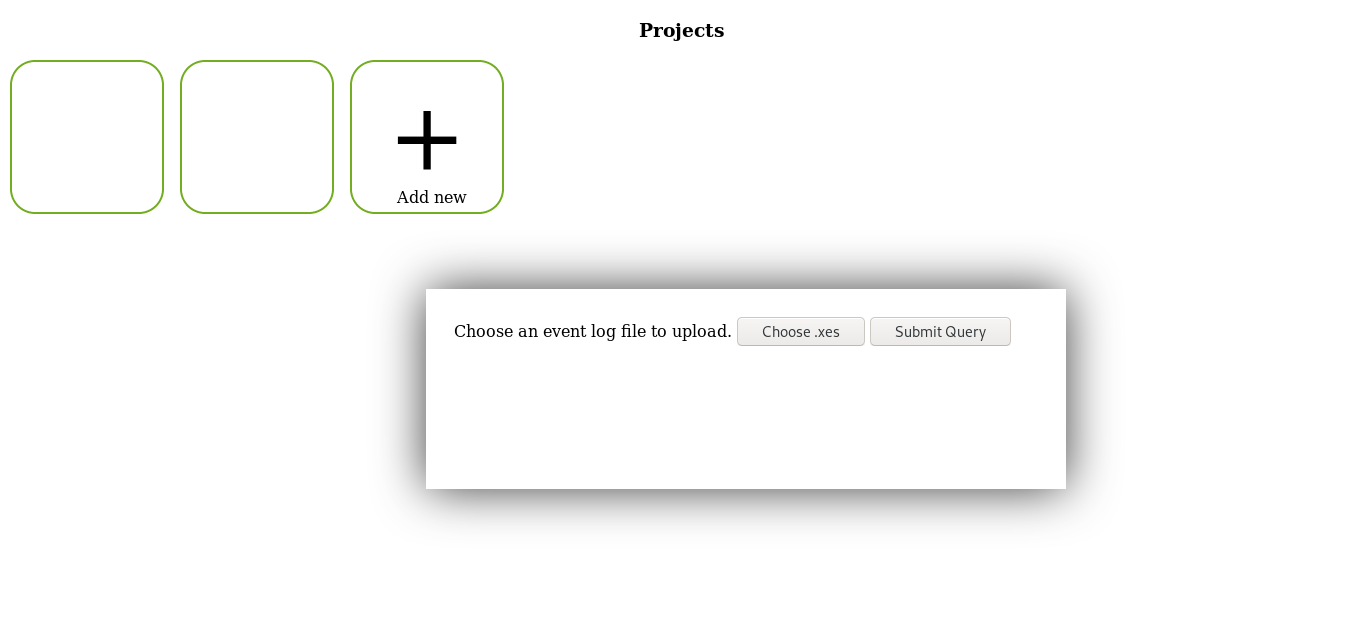
\includegraphics[width=\textwidth]{dummy.png}
    \caption{Mockup of the menu. Here we can add new projects}
    \label{fig:my_label}
\end{figure}

\subsection{Use Case Relations}

\begin{figure}[H]
    \centering
    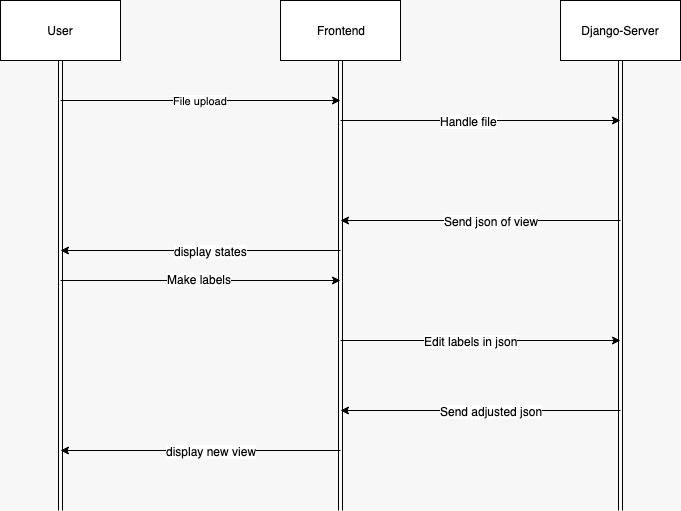
\includegraphics[width=\textwidth]{img1.jpeg}
    \caption{Communication of User, Frontend und Django-Server.}
    \label{fig:arc_1}
\end{figure}


\section{Technical Design}

\subsection{Unit Design: Web Application}

\begin{figure}[H]
    \centering
    \begin{subfigure}[b]{0.85\textwidth}
        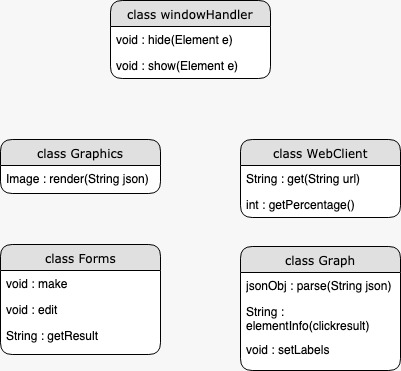
\includegraphics[width=\textwidth]{img3.jpeg}
        \label{fig:arc_1}
    \end{subfigure}
\end{figure}

\subsubsection{windowHandler}
Description: This class will be able to show and hide HTML Objects. \\ \\
Operations: \\
    void: hide(Element e) \\
    Arguments: An HTML Object \\
	Returns: Nothing returned. \\
	Description: This method will hide the HTML Element e. \\ \\
	void: show(Element e) \\
    Arguments: An HTML Object \\
	Returns: Nothing returned. \\
	Description: This method will show the HTML Element e. \\

\subsubsection{Graphics}
Description: This class will render the graphs. \\ \\
Operations: \\
    Image: render(String json) \\
    Arguments: A json file \\
	Returns: The rendered image of the graph defined in the json file. \\
	Description: This method will geneare a graph according to the json file. \\

\subsubsection{Forms}
Description: This class will handle the forms used. \\ \\
Operations: \\
    void: make() \\
    Arguments: None. \\
	Returns: Nothing returned. \\
	Description: This method will generate a form. \\ \\
	void: edit() \\
    Arguments: None. \\
	Returns: Nothing returned. \\
	Description: This method will edit the appearance of a form. \\ \\
	String: getResult() \\
    Arguments: None. \\
	Returns: A String containing the content of a form. \\
	Description: This method will return the content of a form. \\

\subsubsection{WebClient}
Description: This class will receive the data from the back-end. \\ \\
Operations: \\
    String: get(String url) \\
    Arguments: A String containing the url. \\
	Returns: Returns a json file. \\
	Description: This method will return a json file form the url as a String. \\ \\
	int: getPercentage() \\
    Arguments: None. \\
	Returns: A percentage of the download status. \\
	Description: This method will calculate the current download status and return the percentage. \\

\subsubsection{Graph}
Description: This class will represent a graph. \\ \\
Operations: \\
    jsonObj: parse(String json) \\
    Arguments: A json file. \\
	Returns: A json object. \\
	Description: This method will generate the graph according to the json file and will return a json Object. \\ \\
	String: elementInfo(clickresult) \\
    Arguments: The object the user clicked on. \\
	Returns: The information the user demands. \\
	Description: This method will return the information associated to the object the user clicked on. \\ \\
	void: setLabels() \\
    Arguments: None. \\
	Returns: Nothing returned. \\
	Description: This method will make a webRequest to edit a label in a graph. \\
	
	
\subsection{Unit Design: URLs}

\begin{figure}[H]
    \centering
    \begin{subfigure}[b]{0.35\textwidth}
        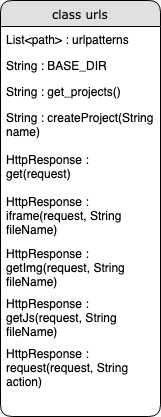
\includegraphics[width=\textwidth]{img2.jpeg}
        \label{fig:arc_1}
    \end{subfigure}
\end{figure}

\subsubsection{urls}
Description: This class will generate responses to received HttpRequests. \\ \\
Attributes:
    String BASE\textunderscore DIR \\
    Description: The String will contain the server directory.
Operations: \\
	String: get\textunderscore projects() \\
    Arguments: None. \\
	Returns: Returns a merged list as a String. \\
	Description: This method will merge all project json files and return it as a String. \\ \\
	String: createProject(String name) \\
    Arguments: The name of the project as a String. \\
	Returns: XXX. \\
	Description: This method will create a new project with a custom name. \\ \\
	HttpResponse: get(request) \\
    Arguments: A request. \\
	Returns: Returns the index.html. \\
	Description: This method will handle all the requests. \\ \\
	HttpResponse: iFrame(request, String fileName) \\
    Arguments: The request and the name of the file. \\
	Returns: Returns a html file. \\
	Description: This method will return a html file used for iframes. \\ \\
	HttpResponse: getImg(request, String fileName) \\
    Arguments: The request and the name of the file. \\
	Returns: Returns a png file. \\
	Description: This method will return a png image from the image folder. \\ \\
	HttpResponse: getJs(request, String fileName) \\
    Arguments: The request and the name of the file. \\
	Returns: Returns a js file. \\
	Description: This method will return a js file used for external resources. \\ \\
	HttpResponse: request(request, String fileName) \\
    Arguments: The request and the name of the file. \\
	Returns: Returns a json file. \\
	Description: This method will generate a json file for a request (e. g. generate Graph, labeling, etc.). \\

\subsection{Unit Design: Back-End}

\subsubsection{Class Structure}

\begin{figure}[H]
    \centering
    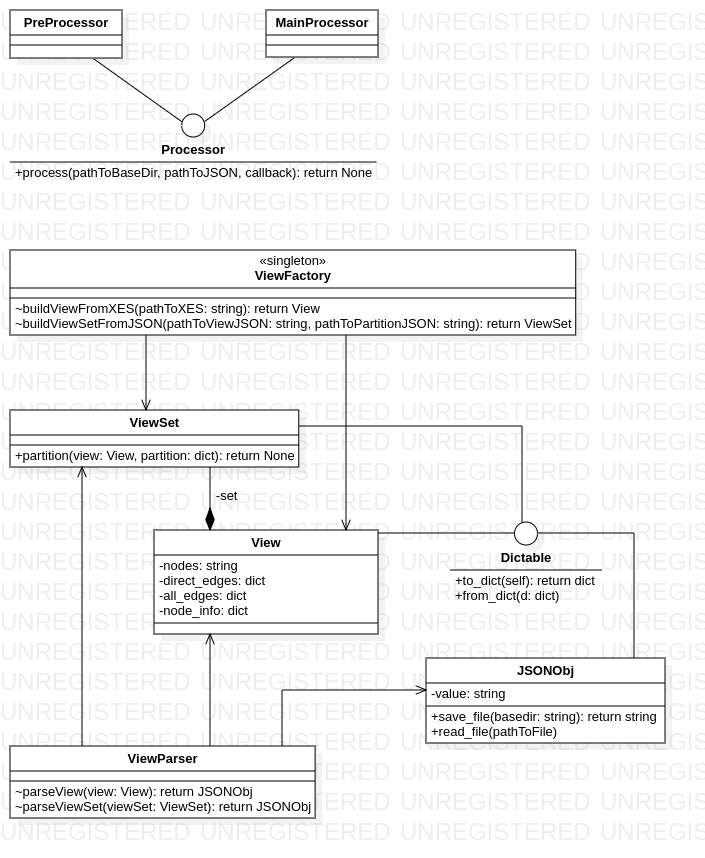
\includegraphics[width=\textwidth]{bclasses.png}
    \caption{Class structure of the backend. Interfaces are depicted with a white circle. Compositions with a black rhombus
    and associations with a standard arrow.}
    \label{fig:bclasses}
\end{figure}

\subsection{Class specification}

\subsubsection{Interface: Processor}

This interface serves as the main entry point of the backend.

\begin{lstlisting}
Attributes: None


Methods:
    + process:
        description:
            this method process a user query of the backend asynchronously by executing a callback function in the end.
            
        parameters:
            pathToBaseDir: string
                path to working directory of the current project context
            pathToJSON: string
                path the the JSON file
            callback : method
                callback function to inform the frontend of succeded process termination and path to relevant files
                
        returns: None
\end{lstlisting}

\subsubsection{MainProcessor}

This class implements the Processor interface. It comes to use when the state partitioning has been chosen by the user and the views are to be computed.

\subsubsection{PreProcessor}

This class implements the Processor interface. It comes to use when the XES file is first uploaded and a graphical representation is done.

\subsubsection{ViewFactory}

This class is a singleton and serves the building of View and ViewSet objects.

\begin{lstlisting}
Attributes: none

Methods:
    + buildViewFromXES:
        description: 
            Parses and analyzes an XES file statistically in order to build a preliminary View object.
        
        parameters:
            pathToXES: string
                path to the XES file to be processed
       
        returns: View
            a view object representing a directly-follows graph derived from the log file
            
    + buildViewSetFromJSON
        description:
            rebuilds the graph that has been preprocessed and turned into a JSON file and partitions it according to the second JSON file
            
        parameter:
        pathToViewJSON: string
            path to the JSON file that rebuilds the preliminary graph
        pathToPartitionJSON: string 
            path to the JSON file that holds the partitioning of the states into views
        
        return: ViewSet
            an appropriate partitioning of the preliminary view 
\end{lstlisting}

\subsubsection{View}

This class represents a directly follows graph.


\begin{lstlisting}
Attributes:
    - nodes: string   
        a list of strings representing the states
        
    - direct_edges: dict
        a dictionary where the keys are nodes and the values are again dictionaries where the keys are the direct successors of the states and the values are their relative frequency of occurrence
        
    - all_edges: dict    
        a dictionary where the keys are nodes and the values are again dictionaries where the keys are all (direct and indirect) successors of the state and the value their relative frequency of occurrence
    
    - node_info: dict
        a dictionary where the keys are nodes and the values are lists of tupels where the first value is the identifier of some statistical information and the second one is the value of that information about the node

Methods: none
\end{lstlisting}

\subsubsection{ViewSet}

A composite class of several views.

\begin{lstlisting}
Attributes:
    - views: View
        a list of views
        
Methods:
    + partition:
        description:
            given a View object and a partitioning, a corresponding set of views is found where edges between views are erased. This method populates the ViewSet object
        
        parameters:
            view: View
                the view to be partitioned
            
            partition: dict
                a dictionary where each node is mapped to a new view label
        
        returns:
            None
\end{lstlisting}

\subsubsection{Interface: Dictable}

Interface that prescribes its realizing classes to be constructable from a dictionary object and to be dumpable to a dictionary object.

\begin{lstlisting}
Methods:
    + to_dict:
        description:
            turns the object into a dictionary
        
        parameter: None
        
        returns: dict
            a dictionary

    + from_dict:
        description:
            populates the object from a dictionary
        
        parameter: 
            d: dict
                a dictionary from which the object is populated
        
        returns: None
\end{lstlisting}


\subsubsection{JSONObj}

This class represents a JSON file and implements the Dictable interface. It is also saveable and it can be populated by reading from a file.

\begin{lstlisting}
Attributes:
    - value: string
        a string representing the content of a JSON file
        
        
Methods:
    + save_file:
        description:
            saves the JSON file to the specified base directory
            
        parameters:
            basedir: string
                directory where the file should be saved
        
        returns: string
            the path to the file as a string
            
    + read_file:
        description:
            populates the JSON object from a file
            
        parameters:
            pathToFile: string
                path to the file that should be read from
                
        returns: None
\end{lstlisting}

\subsubsection{ViewParser}

This class provides methods to parse View and ViewSet objects and turn them in to JSON objects.

\begin{lstlisting}
Attributes: None

Methods:
    ~ parseView:
        description:
            parses a View object and constructs a representation as a JSON object
            
        parameters:
            view: View
                view to be transformed to JSON
        
        returns: JSON
            the corresponding JSON object
            
    ~ parseViewSet:
        description:
            parses a ViewSet object and constructs a representation as a JSON object
            
        parameters:
            viewSet: ViewSet
                ViewSet to be transformed to JSON
        
        returns: JSON
            the corresponding JSON object
\end{lstlisting}

\subsection{Use Case realizations}

\begin{figure}[H]
    \centering
    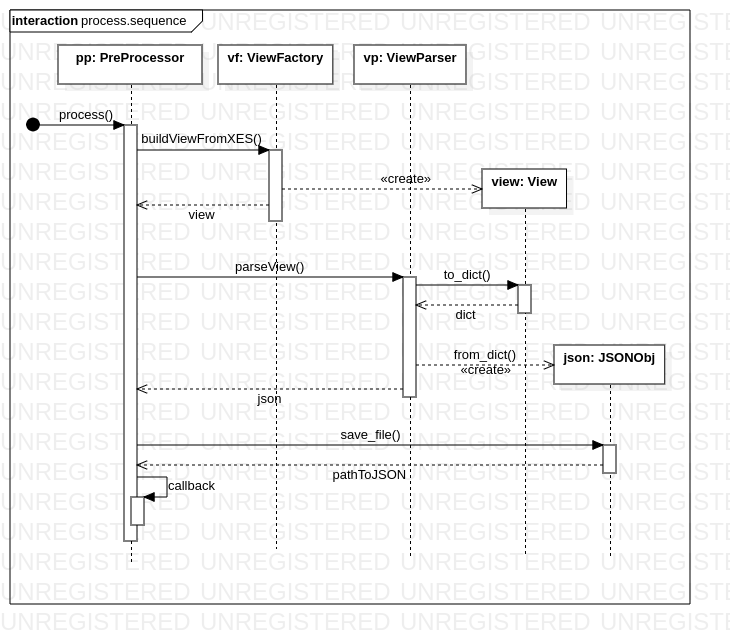
\includegraphics[width=\textwidth]{presequence.png}
    \caption{Use case realization of the call of the process function of the PreProcessor object. A preliminary view is constructed in the end and by the callback function passed back to the frontend component.}
    \label{fig:presequence}
\end{figure}

\begin{figure}[H]
    \centering
    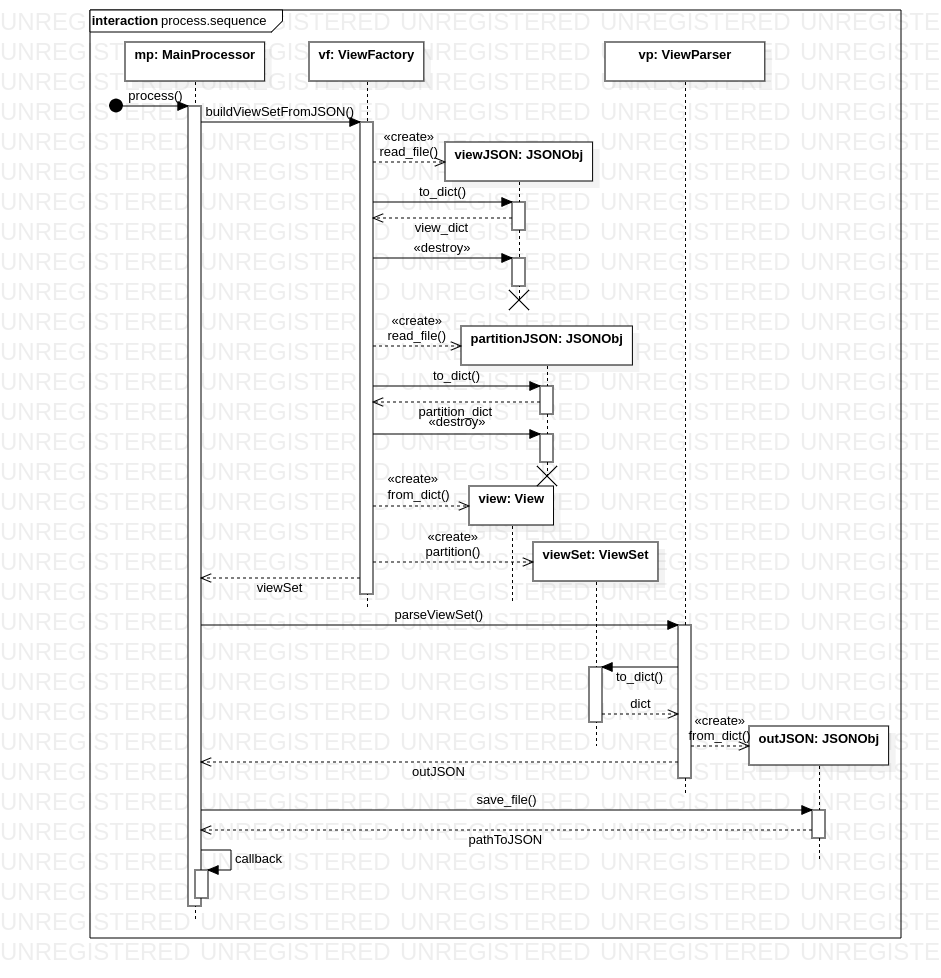
\includegraphics[width=\textwidth]{mainsequence.png}
    \caption{Use case realization of the call of the process function of the MainProcessor object. A set of views is constructed in the end and by the callback function passed back to the frontend component. This set of views hold all the statistical informations of each state and direct and indirect transition between states.}
    \label{fig:mainsequence}
\end{figure}

\end{document}
